    
                %\title{LaTeX Portrait Poster Template}
%%%%%%%%%%%%%%%%%%%%%%%%%%%%%%%%%%%%%%%%%
% a0poster Portrait Poster
% LaTeX Template
% Version 1.0 (22/06/13)
%
% The a0poster class was created by:
% Gerlinde Kettl and Matthias Weiser (tex@kettl.de)
% 
% This template has been downloaded from:
% http://www.LaTeXTemplates.com
%
% License:
% CC BY-NC-SA 3.0 (http://creativecommons.org/licenses/by-nc-sa/3.0/)
%
%%%%%%%%%%%%%%%%%%%%%%%%%%%%%%%%%%%%%%%%%

%----------------------------------------------------------------------------------------
%   PACKAGES AND OTHER DOCUMENT CONFIGURATIONS
%----------------------------------------------------------------------------------------

\documentclass[a0,portrait]{a0poster}
%\setlength{\paperwidth}{33.1in}
%\setlength{\paperheight}{23.4in}

\usepackage[dutch]{babel}
\usepackage{enumitem}
\usepackage{apacite}
\renewcommand\bibliographytypesize{\tiny}
\usepackage{multicol} % This is so we can have multiple columns of text side-by-side
\columnsep=50pt % This is the amount of white space between the columns in the poster
\columnseprule=3pt % This is the thickness of the black line between the columns in the poster

\usepackage[svgnames]{xcolor} % Specify colors by their 'svgnames', for a full list of all colors available see here: http://www.latextemplates.com/svgnames-colors

\usepackage{times} % Use the times font
%\usepackage{palatino} % Uncomment to use the Palatino font

\usepackage{graphicx} % Required for including images
\usepackage{booktabs} % Top and bottom rules for table
\usepackage[font=small,labelfont=bf]{caption} % Required for specifying captions to tables and figures
\usepackage{amsfonts, amsmath, amsthm, amssymb} % For math fonts, symbols and environments
\usepackage{wrapfig} % Allows wrapping text around tables and figures


\begin{document}

%----------------------------------------------------------------------------------------
%   POSTER HEADER 
%----------------------------------------------------------------------------------------

% The header is divided into two boxes:
% The first is 75% wide and houses the title, subtitle, names, university/organization and contact information
% The second is 25% wide and houses a logo for your university/organization or a photo of you
% The widths of these boxes can be easily edited to accommodate your content as you see fit

\begin{minipage}[b]{0.80\linewidth}
\large \color{NavyBlue} \textbf{Bewustzijn heeft aandacht nodig} \color{Black}\\ % Title
\large\textit{Gistperceptie onder dualtaskcondities}\\[2.4cm] % Subtitle
\normalsize \textbf{Raoul Grouls\textsuperscript{1},
	\,Libby van den Besselaar\textsuperscript{2},
	\,Eva Bakels\textsuperscript{3},
	\,Kiki von Piekartz\textsuperscript{4}}\\[0.5cm] % Author(s)
\small Universiteit Utrecht,\,Kunstmatige Intelligentie,\, Nederland\\[0.4cm] % University/organization
\small \texttt{1 r.h.grouls@students.uu.nl}\\
\texttt{2 l.l.m.vandenbesselaar@students.uu.n}\\
\texttt{3 e.e.bakels@students.uu.nl}\\
\texttt{4 k.g.piekartz@students.uu.nl}\\
\end{minipage}
%
\begin{minipage}[b]{0.3\linewidth}

\includegraphics[width=12cm]{uu-logo.png}\\ 
\end{minipage}

\vspace{1cm} % A bit of extra whitespace between the header and poster content

%----------------------------------------------------------------------------------------

\begin{multicols}{3} % This is how many columns your poster will be broken into, a portrait poster is generally split into 2 columns

%----------------------------------------------------------------------------------------
%   ABSTRACT
%----------------------------------------------------------------------------------------

\color{Navy} % Navy color for the abstract

\begin{abstract}
bla die bla
\end{abstract}
%----------------------------------------------------------------------------------------
%   INTRODUCTION
%----------------------------------------------------------------------------------------

\color{Black} % SaddleBrown color for the introduction
\section*{Introductie}
Onderzoek heeft overtuigend aangetoond dat \textit{aandacht zonder bewustzijn} mogelijk is \cite{Jiang_Costello_Fang_Huang_He_2006, Sklar_Levy_Goldstein_Mandel_Maril_Hassin_2012, Cohen_Cavanagh_Chun_Nakayama_2012, Reddy_Reddy_Koch_2006, Li_VanRullen_Koch_Perona_2002}. Onderwerp van discussie is de vraag of \textit{bewustzijn zonder aandacht} mogelijk is \cite{Cohen_Cavanagh_Chun_Nakayama_2012,Mack_Clarke_2012, Jennings_2015, Block_2011}. Hierbij wordt onderzoek naar gistperceptie onder dualtask-condities gebruikt: \'{e}\'{e}n taak is ontworpen om de bestaande aandacht te monopoliseren, de andere taak is gistperceptie (het waarnemen van de grote lijnen van een afbeelding die 30ms wordt getoond) \cite{Mack_Clarke_2012}.
\textbf{Aandacht} is daarbij gedefini\"eerd als  \textit{topdown, selectieve aandacht}. Door selectieve aandacht wordt informatie diepgaander verwerkt \cite{Cohen_Cavanagh_Chun_Nakayama_2012}. 
\textbf{Bewustzijn} verwijst naar de inhoud van bewustzijn en expliciet niet naar niveaus van bewustzijn zoals waken of slapen \cite{VanBoxtel_Tsuchiya_Koch_2010}.  

\color{Black} % DarkSlateGray color for the rest of the content

\section*{Hypothese}
De kritiek op het onderzoek naar gistperceptie als onderbouwing voor \textit{bewustzijn zonder aandacht} is dat de aandachtstaak simpelweg niet intensief genoeg is\cite{Cohen_Alvarez_Nakayama_2011, Mack_Clarke_2012}. Deze onderzoeken gebruiken als onafhankelijke variabele een \textit{aandachtsinstructie}. De proefpersonen mogen dan de aandachtstaak compleet los laten, om te zoeken naar de gistafbeelding. Dit is een belangrijke beperking, omdat hiermee oogbewegingen worden ge\"introduceerd die als contaminerende variabele kunnen optreden aangezien proefpersonen in de periferie minder detail waarnemen dan in het centrum van de blik\cite{moore2013clinically}. Daarom onderzoeken de invloed van variatie in de aandachtstaak op de gistperceptie. Wij hypothetiseren dat:
\begin{quote}
\textit{Wanneer aandacht een voorwaarde is voor bewustzijn, dan moet een aandachtstaak die toeneemt qua intensiteit leiden tot een verminderd bewustzijn van de gist. Wanneer aandacht geen voorwaarde is voor bewustzijn, zal het het bewustzijn van de gist gelijk blijven.}
\end{quote}
\begin{center}\vspace{1cm}
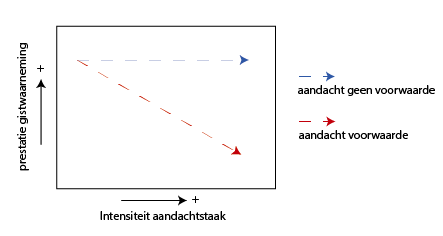
\includegraphics[width=1.0\linewidth]{illustratieHypothese.png}
\captionof{figure}{\color{Green} De visualisatie van onze hypothese. Of aandacht een voorwaarde is voor bewustzijn wordt zichtbaar in de correlatie tussen gistperceptie en intensiteit van de aandachtstaak.}
\end{center}%\vspace{1cm}
%----------------------------------------------------------------------------------------
%   GEOTHERMAL DATA
%----------------------------------------------------------------------------------------
\section*{Methode}
We hebben voor ons onderzoek de globale opzet van o.a. Mack \& Clarke (2012), Reddy et al. (2006) en Li et al. (2002) gebruikt: een dual-task opzet met een centrale aandachtstaak en perifere gistperceptie. Voor een aandachtstaak die schaalbaar is qua intensiteit hebben we de opzet met een \textit{multiple-object tracking task} overgenomen van Alvarez en Oliva (2008)\nocite{Alvarez_Oliva_2008}.\\
\textbf{Participanten} We hebben bij de selectie van proefpersonen (n=34) gestreefd naar een spreiding van leeftijd en evenwichtige man/vrouw verhouding.(zie tabel 1). 
\captionof{table}{Demografie van de proefpersonen}
\begin{center}
\begin{tabular}{r r r r r r} 
	\hline
	leeftijd (mediaan) & SD & min & max & man/vrouw & aantal \\
	\hline
	22 & 15 & 17 & 60 & 17/17 & 34\\
	\hline
\end{tabular}
\end{center}
We hebben rekening gehouden met de etniciteit van proefpersonen, omdat we verwachten dat dat mogelijk invloed kan hebben op het herkennen van de gezichten\cite{sporer2001recognizing}. \\
\textbf{Materiaal} Het experiment is opgezet met behulp van PsychoPy2 software\cite{peirce2007psychopy, Peirce2009generating} en geanalyseerd met R\cite{Rsoftware}. De complete code is te vinden op \cite{Grouls2017}.

\begin{center}\vspace{1cm}
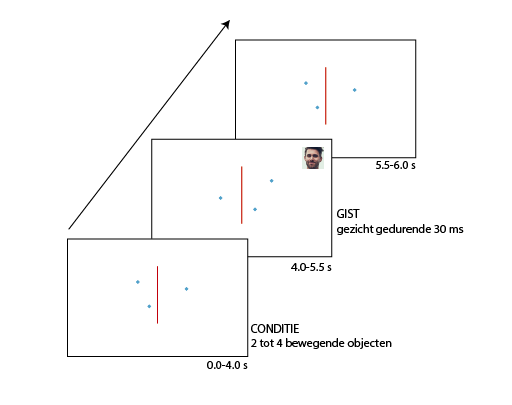
\includegraphics[width=1.0\linewidth]{Methode.png}
\captionof{figure}{\color{Green} (A) Temp. vs. depth for different regions.}
\end{center}\vspace{1cm}

%------------------------------------------------

\subsection*{Resultaten}
\begin{enumerate}
\item The Tlemcenian dolomites in the NW-Algeria: thermal waters are related to the Plio-Quaternary volcanic rocks; bicarbonate water type.
\item Carbonate formations in the NE-Algeria: area is 15,000 km$^2$; high flow rates (\textgreater100 L/s); highest temperature in Algeria (98 $^{\circ}$C). 
\end{enumerate}

\subsection*{Hot Springs}
\begin{center}\vspace{1cm}
	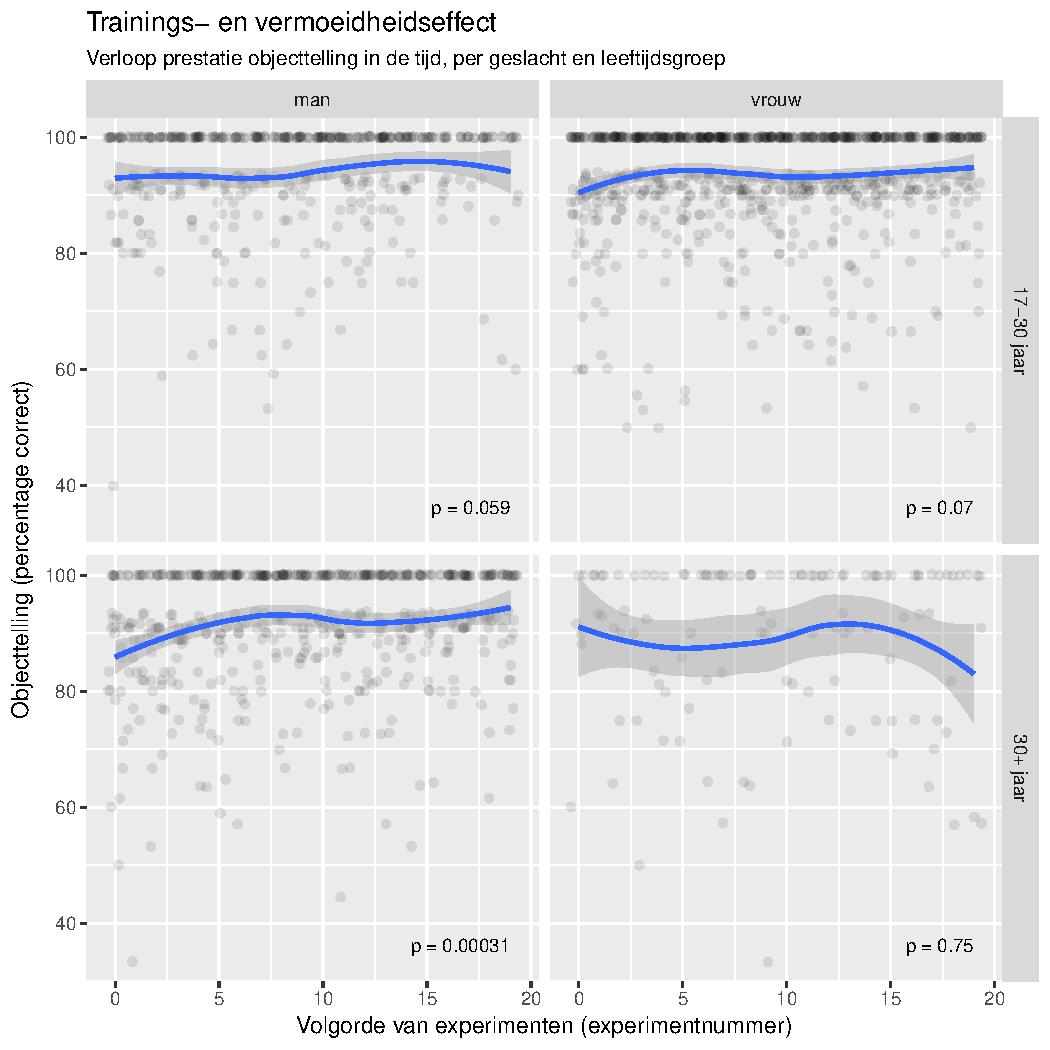
\includegraphics[width=0.8\linewidth]{training-grid.pdf}
	\captionof{figure}{\color{Green} Temperatures of the main hot springs of the northern part of Algeria}
\end{center}\vspace{1cm}
\begin{center}
\begin{tabular}{r r r}
	\hline
	p & c2 & afkap\\
	\hline
	0.07 & -0.03 & 5\\
	0.03 & -0.03 & 8\\
	0.01 & -0.04 & 9\\
	0.01 & -0.03 & 10\\
	0.04 & -0.02 & 15\\
	0.03 & -0.02 & 17\\
	0.02 & -0.03 & 20\\
	\hline
\end{tabular}
\end{center}

\begin{center}\vspace{1cm}
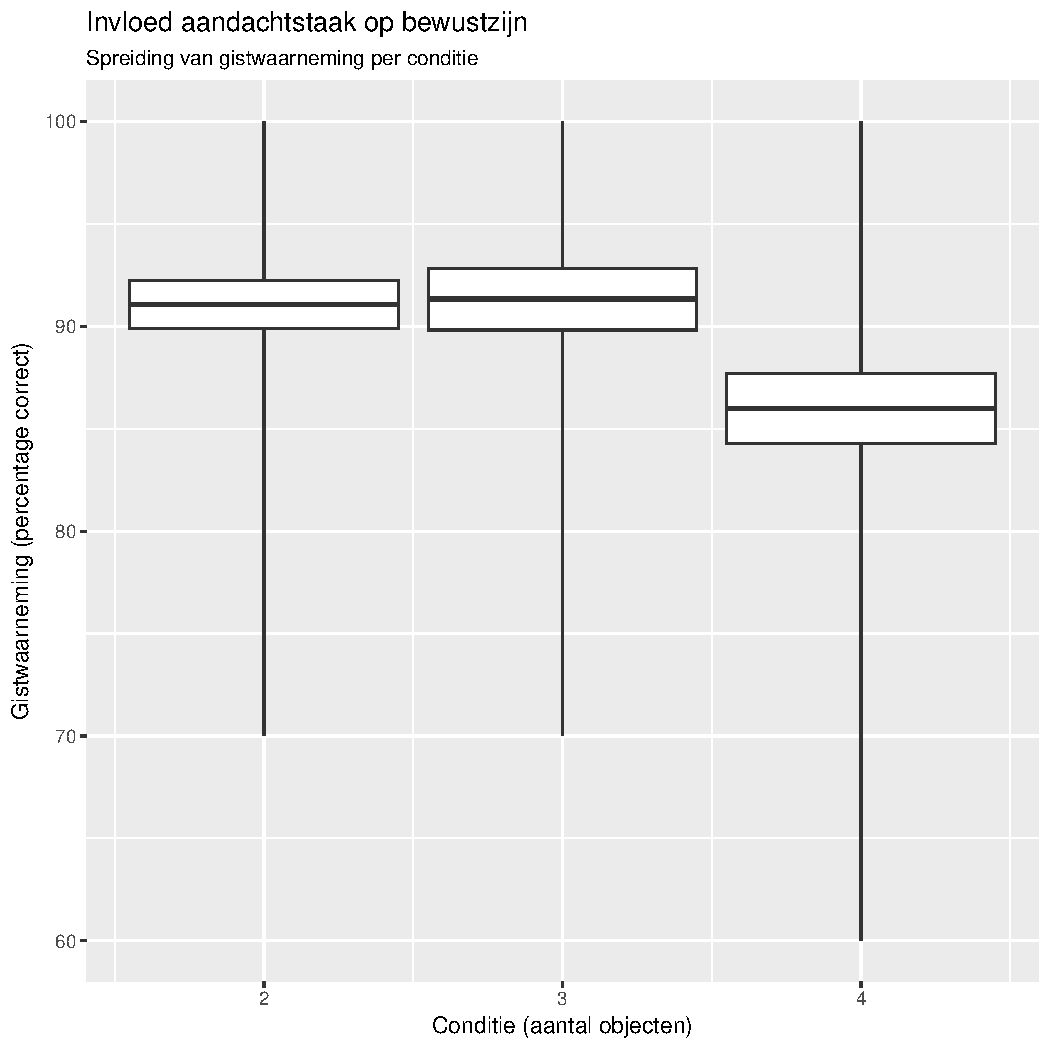
\includegraphics[width=1.0\linewidth]{boxplotGist-conditie.pdf}
\captionof{figure}{\color{Green} (A) Mixing model to illustrate the relative contribution of magmatic, meteoric and crustal sources of gases in NE Algerian geothermal discharges. (B) Photo of the concretions of Hammam Meskhoutine (NE Algeria). The height of the concretions on successive conduits reaches 30 m.}
\end{center}\vspace{1cm}

\begin{center}\vspace{1cm}
	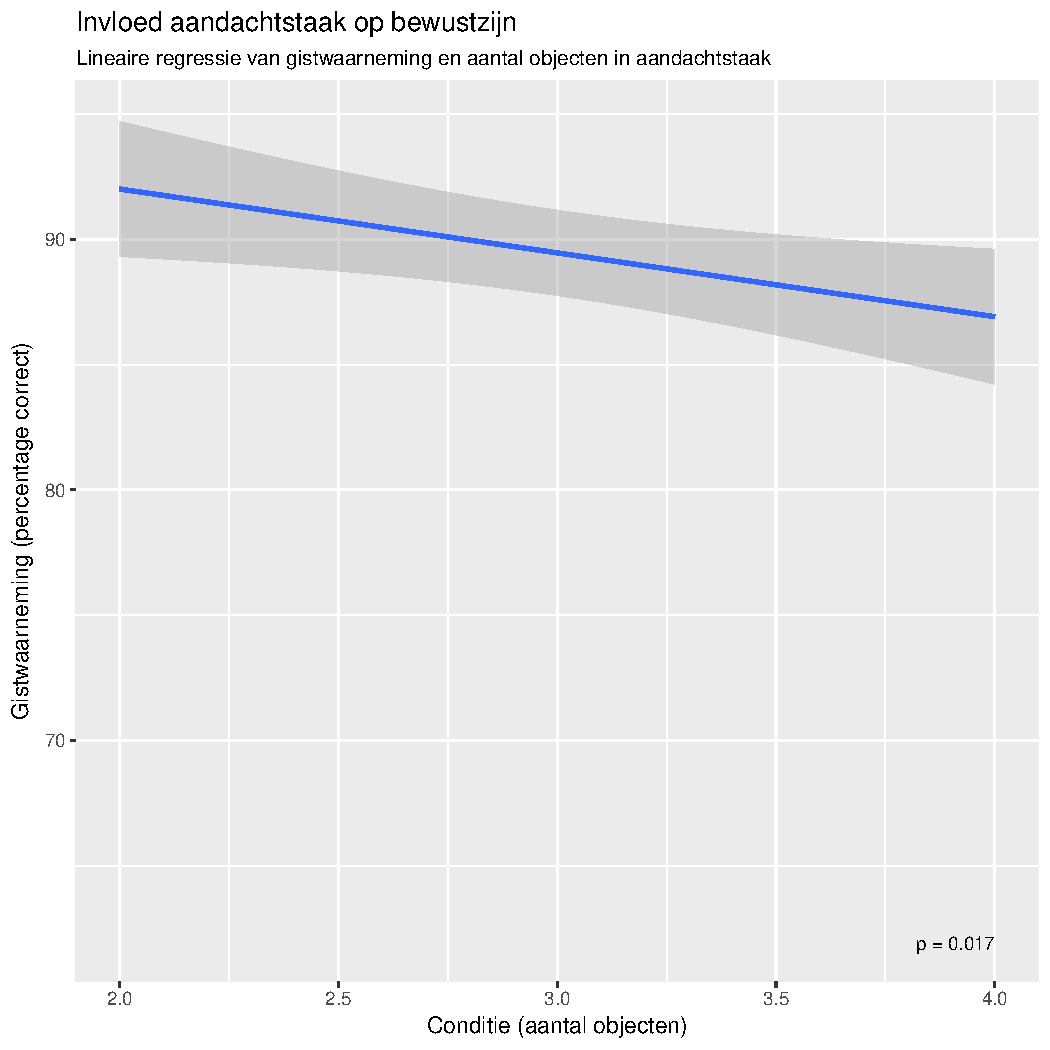
\includegraphics[width=0.8\linewidth]{lineaireRegressie.pdf}
	\captionof{figure}{\color{Green} Location of Algerian geothermal uses sites}
\end{center}\vspace{1cm}

\subsection*{Discussie}
\begin{itemize}
\item Utilizations of the hot water in Algeria are balneology, space and greenhouse heating. 
\item Heat-pump in a primary school (NW Algeria) for heating and cooling purposes.
\item Tilapia fish farming in south of Algeria (Ghardaia and Ouargla).
\item Greenhouses for melon and tomato cultivation in South of Algeria (Ouargla and Touggourt).
\item Future projects: binary-cycle geothermal power plant in Guelma (NE-Algeria); heat-pump in Khenchla (NE Algeria).
\end{itemize}
The total energy use for geothermal is about 1,778.65 TJ/yr.





%----------------------------------------------------------------------------------------
%   CONCLUSIONS
%----------------------------------------------------------------------------------------

\color{SaddleBrown} % SaddleBrown color for the conclusions to make them stand out

\section*{Conclusies}
Despite being a petroleum- and gas-rich country, 
\color{Black} % Set the color back to DarkSlateGray for the rest of the content

%----------------------------------------------------------------------------------------
%   FORTHCOMING RESEARCH
%----------------------------------------------------------------------------------------


 %----------------------------------------------------------------------------------------
%   REFERENCES
%----------------------------------------------------------------------------------------


%----------------------------------------------------------------------------------------
\bibliographystyle{apacite}
\bibliography{biblio}
\end{multicols}
\end{document}
              
            